\begin{frame}
	\frametitle{Kipppunkte des Klimasystems}
	\begin{figure}
		\centering
		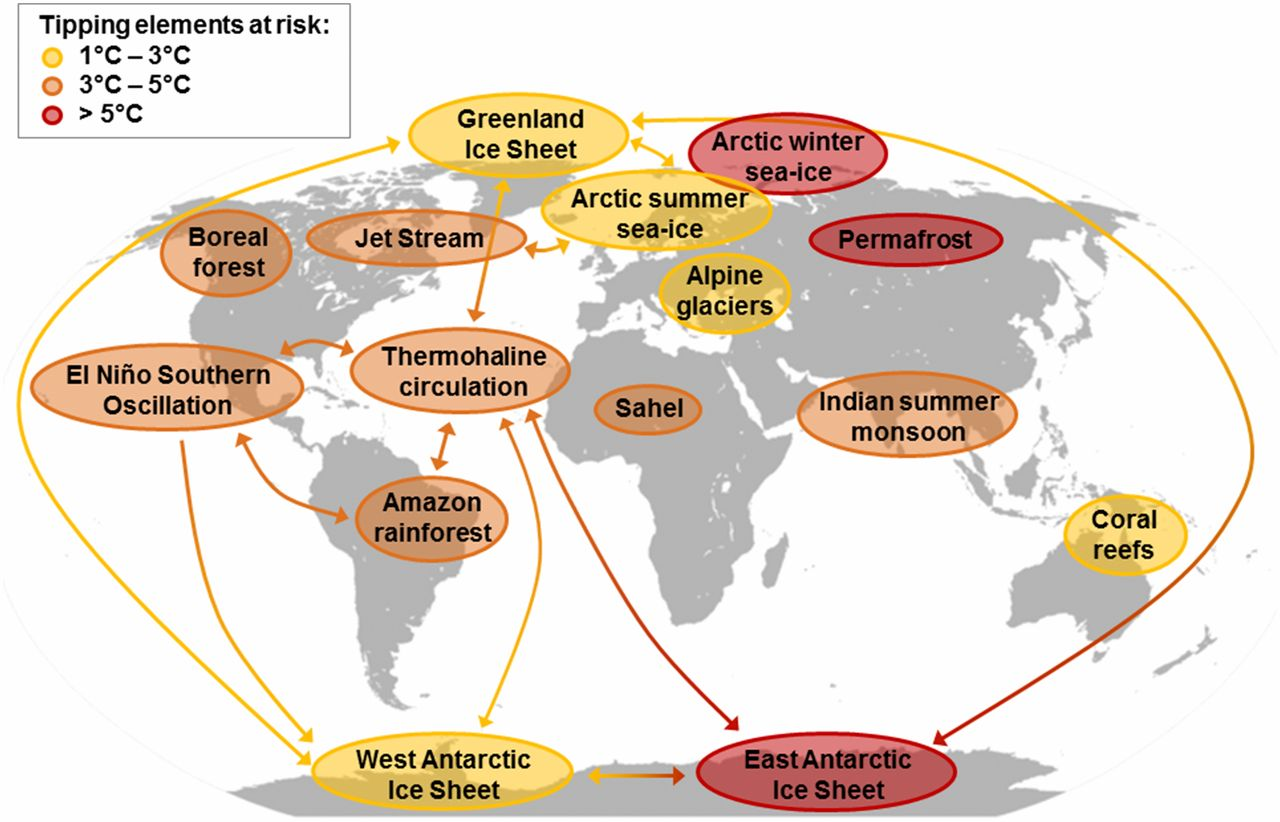
\includegraphics[width=0.9\linewidth]{bilder/tipping_elements}
		\caption{Die wichtigsten bekannten möglichen Kipppunkte unseres Klimasystems aus [Len]}
		\label{fig:tippingelements}
	\end{figure}

	\note{
	\begin{itemize}
		\item[] Für kleine Änderungen ist der Zusammenhang zwischen anstieg der Treibhausgaskonzentration und anstieg der Temperatur nahezu proportional
		\item [] Es gibt aber auch Effekte, die sich auf Wetter und Klima auswirken, welche sich aber einer gewissen Temperatur selbst verstärken -> Wir haben das in Form der Eis-Albedo-Rückkoplung schon kurz angesprochen
		\item[] Auch die thermohaline Zirkulation der Wassermassen ist ein Beispiel dafür, da diese ja gerade durch die Wassertemperatur angetrieben wird. Änderungen der Zirkulation können dann zu lokalen Änderungen des Klimas führen
		\item[] Selbstverstärkende Effekte haben die Eigenschaft ab einem gewissen Punkt kaum noch aufhaltbar zu sein, man spricht daher von \textit{Kipppunkten} im Klimasystem.
		\item[] Sowohl die Zeitskala auf der so ein Effekt abläuft (siehe Trägheit), als auch die Temperatur ab der dieser einsetzen kann, ist für jeden Kippunkt unterschiedlich
		\item [] \glqq Das Klimasystem ist kein träges und gutmütiges Faultier, sondern es kann sehr abrupt und heftig reagieren\grqq [UBA]
		\item I.A. sind diese Kipppunkte deutlich schwerer zu modelieren, da ihre Folgen beim eintreten massiv sind, und sie sich in einer Art Kettenreaktion auch gegenseitig auslösen können (Pfeile in Abbildung).
	\end{itemize}
}
\end{frame}

\begin{frame}
	\frametitle{Beispiele für Kipppunkte des Klimasystems}
	\begin{columns}
		\column[t]{0.5\linewidth}
		\begin{figure}
			\centering
			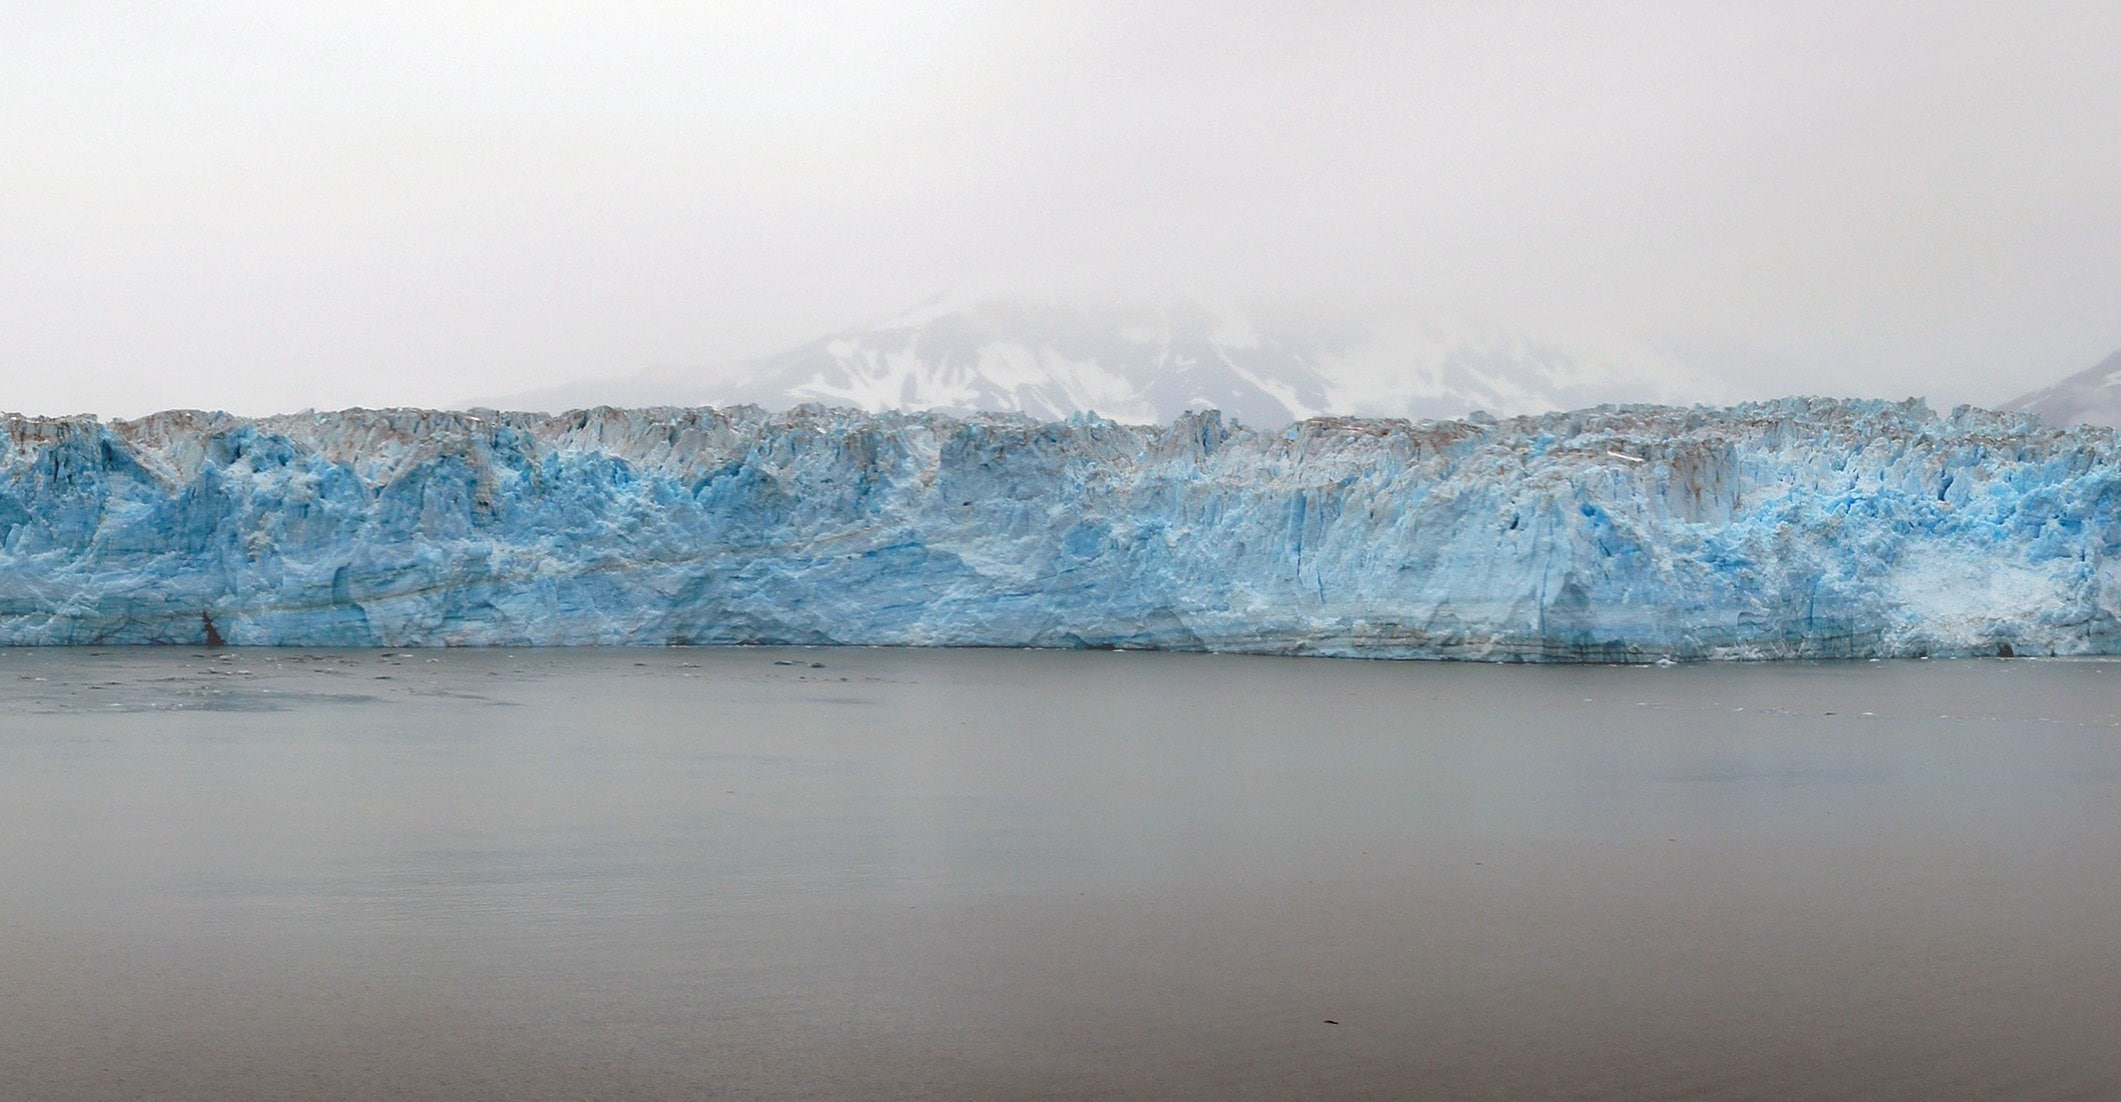
\includegraphics[width=0.9\linewidth]{bilder/groenland}
			\caption{Eisschild auf Grönland}
			\end{figure}
		\begin{itemize}
		\item Wenn der Kilometer dicke Eispanzer auf Grönland schmilzt, könnte der Meeresspiegel um bis zu 7 Meter steigen

		\end{itemize}
		\column[t]{0.5\linewidth}
		\begin{figure}
			\centering
			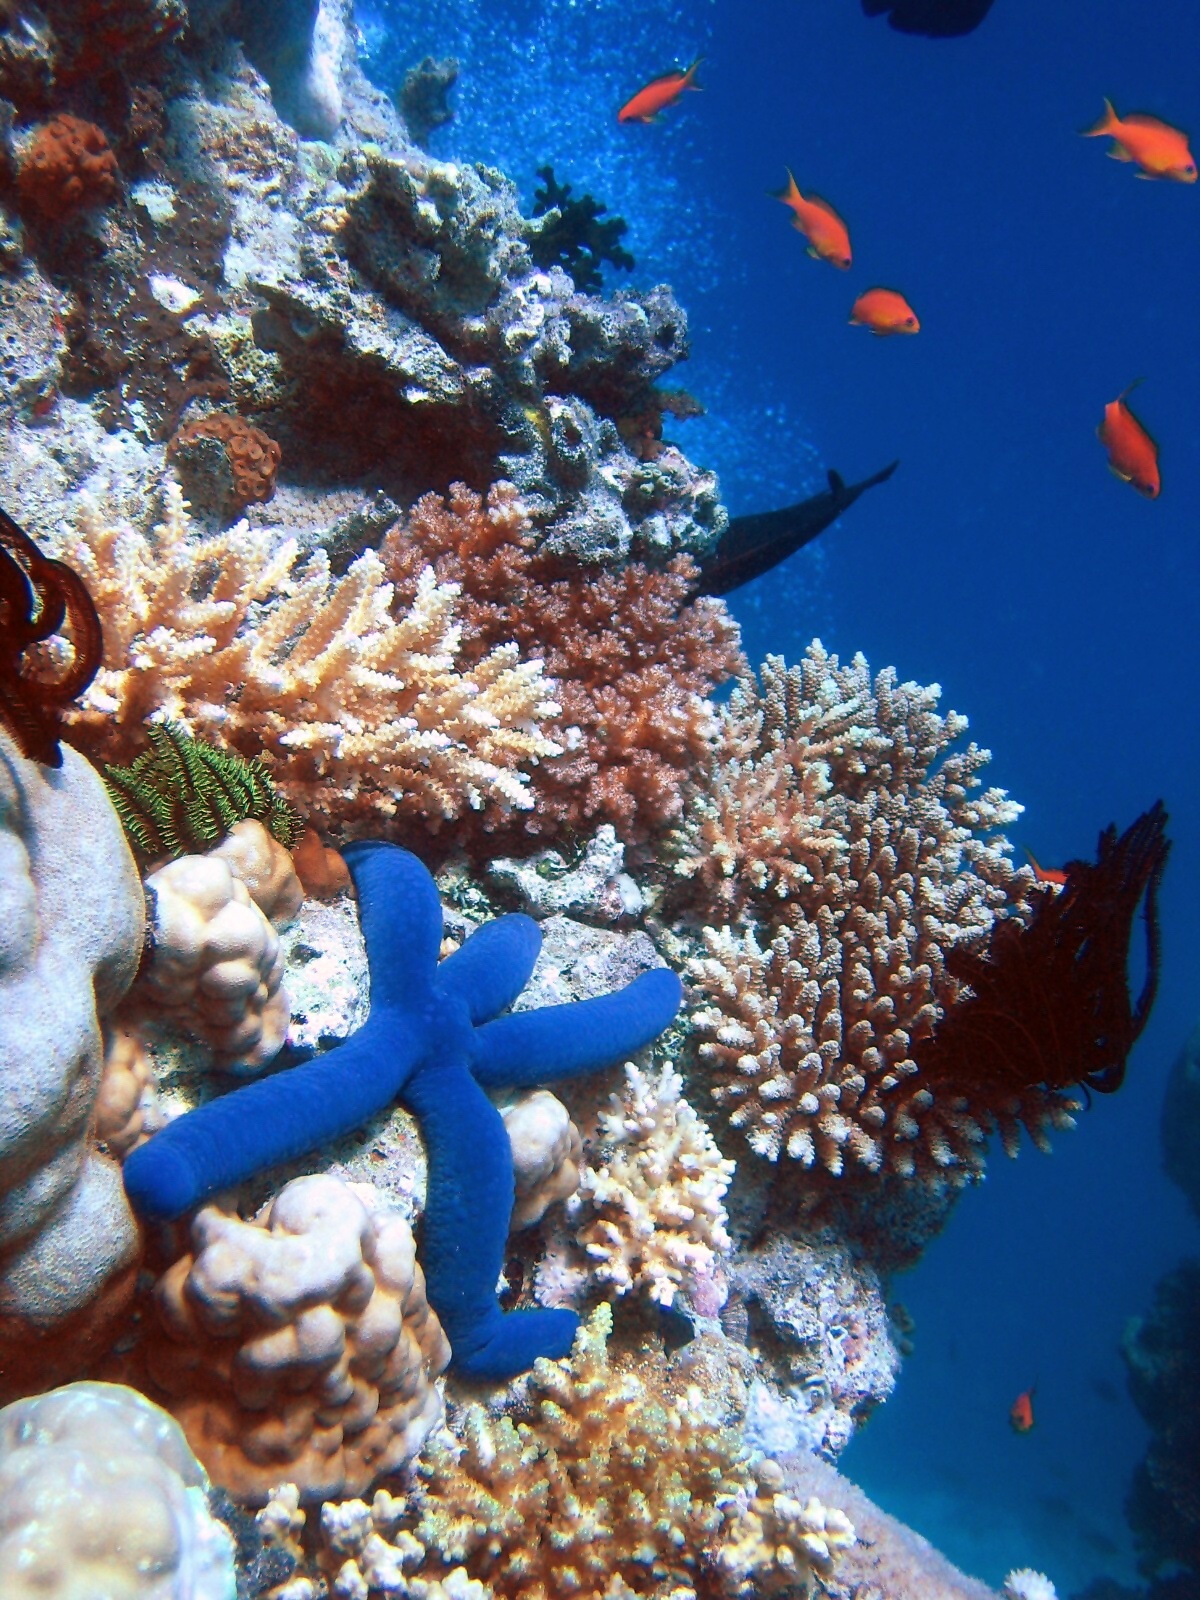
\includegraphics[height=0.9\linewidth, angle=90]{bilder/great_barrier_reef}
			\caption{Korallen vor Australien}
		\end{figure}
		\begin{itemize}
			\item Die weltweiten Korallenriffe leiden unter Versauerung der Ozeane und erhöhter Temperatur
		\end{itemize}
	\end{columns}


	\note{
		\begin{itemize}
		\item[] Grönland ist auf einer Fläche von \SI{1.8e6}{\kilo\meter\squared} (etwa 5 mal Deutschland) mit einem bis zum \SI{3}{\kilo\meter} dicken Eispanzer bedeckt.
		\item[] Der Eispanzer unterliegt durch Schmelzen im Sommer und Schneefall einer ständigen Veränderung.
		\item[] Außerdem geht an den Küsten kontinuierlich Eis verloren.
		\item[] Bei höheren Temperaturen wird das Wechselspiel aus Schmelzen und Wachstum gestört, außerdem gleitet das Eis auf Schmelzwasser schneller ins Meer
		\item[] In Folge kann es zu einem raschen abschmelzen kommen und dadurch bedingt zu einem Anstieg des Meeresspiegels um bis zu \SI{7}{\meter} über Jahrhunderte
		\item[] Dieser Kipppunkt könnte bereits erreicht sein [King]. Auch eine sofortiger Stopp der globalen Temperaturerhöhung würde das abschmelzen dann nicht mehr verhindern.
		\item[] Das Eis in der Westantartikis verhält sich ähnlich, könnte jedoch etwas stabiler sein, dass Eis in der Ostantarktis scheint bisher weniger gefährdet
		\item[] Durch Erhöhung des CO2 Gehaltes wird das Meerwasser langsam sauer. Das wirkt sich negativ auf viele Lebewesen aus, insbesondere Korallen, da in sauerer Umgeubg nicht genug Kalk zur Verfügung steht.
		\item[] Die höheren Temperaturen führen außerdem vermehrt zur Korallenbleiche. Bei dieser sterben die Algen auf der Oberfläche der Korallen ab, was die Koralle selbst ebenfalls schädigt.
		\item[] Ab einem gewissen Grad der Schädigung werden die Korallenriffe zunehmende absterben, selbst wenn sich CO2 Gehalt und Temperatur nicht weiter erhöhen.
		\end{itemize}
	}
\end{frame}
